\documentclass[italian, Lau, oneside, nodefaultfont, noexaminfo]{sapthesis}
\usepackage[italian]{babel}
\usepackage[T1]{fontenc}
\usepackage[utf8]{inputenx}
\usepackage{indentfirst}
\usepackage{microtype}
%\usepackage{yfonts,color}
%\usepackage{float}
\usepackage{listings}
\fontsize{15pt}{18pt}
\counterwithout{footnote}{chapter}
\usepackage{url}
\usepackage[chapter]{minted}
\usepackage{lettrine}
\linespread{0.9}
\usepackage{chngcntr}
\usepackage[nottoc, notlof, notlot]{tocbibind}
\usepackage{hyperref}
\hypersetup{
			colorlinks=true,
            linkcolor = black,                      
            linktoc=page,
			anchorcolor=black,
            citecolor= black,
            urlcolor  = black,  		
            pdftitle={relazione-tirocinio-lorenzo-camilli},
			pdfauthor={Lorenzo Camilli},
			pdfkeywords={thesis, sapienza, roma, university} 
}

\title{Progettazione e sviluppo di API per il calcolo di statistiche per l'applicazione GeneroCity}
\author{Lorenzo Camilli}
\IDnumber{1845956}
\course[]{Informatica}
\courseorganizer{Facolt\`a di Ingegneria dell'informazione, informatica e statistica}
\submitdate{2020/2021}
\copyyear{2021}
\advisor{Emanuele Panizzi}
\authoremail{camilli.1845956@studenti.uniroma1.it}
\examdate{}

\begin{document}

\frontmatter
\maketitle
\begin{abstract}
Il seguente elaborato presenta il mio percorso di tirocinio svolto presso il Dipartimento di Informatica dell'universit\`a di Roma La Sapienza.

Durante questo percorso ho fatto parte di un gruppo di lavoro che ha progettato una applicazione di \textit{smart parking} denominata \textbf{GeneroCity}, sotto la direzione del prof. Emanuele Panizzi. Per smart-parking si intende l'utilizzo di tecnologie al fine di individuare facilmente e in tempo reale i parcheggi disponibili in una determinata zona.   Mi sono occupato principalmente dello sviluppo di API (\textit{Application Programming Interface}), ovvero del software che si occupa di fornire funzionalit\`a ad altri componenti, software o hardware. In particolare, in \textbf{GeneroCity} ho lavorato su API necessarie al  calcolo di alcune statistiche di utilizzo dei parcheggi.
Nell'elaborato verranno inizialmente esposte   le conoscenze preliminari, e successivamente si affronter\`a la fase di implementazione e di sviluppo.

\end{abstract}

\tableofcontents

\mainmatter

%=================INRTODUZIONE=========================
\bigskip
\chapter *{Introduzione}

\addcontentsline{toc}{chapter}{Introduzione} 
Secondo il recente  studio di Nomisma, ``Attori e modelli per una mobilità sostenibile'', presentato il 26 maggio 2021, in Italia le automobili ci sono 663 ogni 1000 abitanti, la larga maggioranza della popolazine (64\%)  utilizza quotidianamente  l'auto per i propri spostamenti. La  congestione dei grandi centri urbani fa  perdere nel traffico l’equivalente di oltre 10 giornate lavorative, che diventano 21,5   a Roma e 18,6 a Milano, con conseguenze negative su di noi e sull’ambiente, in termini di stress, qualit\`a dell'aria, spazio pubblico  e inquinamento. Parte di questo tempo \`e speso nella ricerca  di un parcheggio, tempo  che pu\`o arrivare anche a raggiungere svariate decine di minuti. Il problema non \`e solo italiano:  secondo \cite{ref:article-parking}  gli americani spendono circa 17 ore all'anno nella ricerca del parcheggio, negli UK questo dato arriva fino a 44 ore.
Il riuscire a mitigare questo problema con servizi che puntino all'ottimizzazione, tramite strumenti tecnologici,  dell'uso dello spazio pubblico e in particolare dei parcheggi, si inserisce dunque tra  i possibili obbiettivi delle cosidette ``citt\`a intelligenti''.  
L'applicazione \textbf{GeneroCity}, attualmente in fase di studio e sperimentazione da parte di un gruppo di ricercatori e studenti del Dipartimento di Informatica della Sapienza di Roma,  interviene nella  fase del parcheggio  con lo  scopo  di   aiutare l'automobilista  a ridurne i tempi.

L'idea di base dell'applicazione \textbf{GeneroCity} \`e quella di effettuare lo scambio di parcheggio tra utenti. Un utente, detto \textit{giver}, dichiara al sistema che sta lasciando un parcheggio in una data posizione, un altro utente (il \textit{taker}) tramite una segnalazione usando una funzione apposita o mediante attivazione automatica rilevata dall'applicazione (in modo da ridurre l'uso del telefono alla guida), potr\`a usufruire del parcheggio lasciato dal giver. Con questo sistema chi cerca parcheggio non dovr\`a sprecare tempo e benzina  girando a vuoto, ma sapr\`a subito dove andare. L'applicazione non richiede l'introduzione di nuovo hardware, ma   sfrutta  i sensori gi\`a  disponibili  nei telefoni, come il GPS e l'accelerometro, che col passare delle generazioni diventano sempre pi\`u precisi.

Il mio lavoro si \`e concentrato sullo sviluppo di funzionalit\`a (\autoref{sec:api}) che implementino la sezione delle statistiche inerenti il tempo e  la distanza di ricerca dello stallo. Queste funzionalit\`a  vengono  integrate nell'applicazione, in modo da restituire un feedback immediato all'utente sui vantaggi dell'uso dell'app.
\\

 Una volta stabilito l'obbiettivo da realizzare con le API (costruzione delle statistiche di tempi e distanze di ricerca dei parcheggi) ho analizzato le informazioni a mia disposizione fornite del sistema per capire quali tra i dati mi sarebbero stati utili e che quindi  avrei dovuto estrapolare. Successivamente sono passato alla fase di progettazione, che include anche la definizione di possibili condizioni di errore di raccolta dati e conseguente notifica all'utente. Dopo questa prima fase di studio,  ho affrontato   lo sviluppo vero e proprio delle API, terminato il quale sono passato ad una fase di test. 
 
La relazione \`e composta come segue. 

Nel \autoref{cap:cap02} vengono affrontati gli strumenti che sono stati usati, ai fini dello  sviluppo del progetto.\\

Nel \autoref{cap:cap03} \`e  esposta una parte teorica in cui sono presentate cosa sono le API e come funzionano. Un paragrafo è dedicato al protocollo HTTP, parte fondamentale di una API. Viene quindi esposta la struttura dell'applicazione GeneroCity e le sue funzionalit\`a principali. La parte finale affronta nel dettaglio il lavoro da me svolto, in particolare la fase di progettazione delle API. \\

Infine,  il  \autoref{cap:cap04} tratta lo sviluppo delle API dell' applicazione \textbf{GeneroCity}, i calcoli che esse effettuano sui dati del sistema, la loro interazione con il database e come esse reagiscono alle varie condizioni.\\

%%%DA SPOSTARE NELLA SEZIONE APPOSITA (ALLA FINE, se proprio devo)
%\\Concludo ringraziando mia madre e mio padre, mia sorella, che mi hanno sempre incoraggiato, con la loro presenza, la loro fiducia, la loro severit\`a mista all'ironia. Ringrazio la mia amica di sempre Ivana, e i miei amici e  colleghi Vincenzo e Gaetano, che con il loro aiuto prezioso mi hanno permesso di superare momenti difficili nello studio. Ringrazio il prof. Panizzi per avermi appassionato al lavoro di tirocinio. Ringrazio infine la professoressa Loreti, mia prima professoressa di matematica del liceo, la cui % negativit\`a e mancanza di visione miopia mi  ha stimolato   a fare sempre meglio. 
 


%================Capitolo 2 tecnologie usate=========
\bigskip

\chapter{Architettura e tecnologie}
\label{cap:cap02}

Durante il mio percorso di tirocinio ho avuto l'occasione di sperimentare  tecnologie e protocolli per lo sviluppo del lato back-end del progetto, in particolare il linguaggio di programmazione \textbf{Go}, le piattaforme \textbf{GitLab} e \textbf{Docker} ed il software \textbf{Postman}. Di seguito espongo le motivazioni che hanno portato alla  scelta di questi strumenti rispetto ad altri simili, il loro funzionamento e in che modo sono stati utilizzati.

\section{Go}
Sicuramente parte fondamentale quando si decide di sviluppare un'applicazione, o pi\`u in generale un software, \`e la scelta del linguaggio di programmazione. In questa fase \`e importante avere ben chiari quali siano i requisiti che il software deve rispettare. In  particolare nel caso dell'applicazione GeneroCity si richiedono principalmente reattività, facilit\`a di utilizzo, supporto e stabilit\`a. Pertanto la scelta \`e ricaduta sul linguaggio  open-source con licenza BSD\footnote{ La licenza BSD \`e un tipo di licenza open-source, pi\`u restrittiva della GPL, ovvero quella che lascia la massima libert\`a, che permette a chiunque di modifcare il codice, con l'unico dovere di citare l'autore. Quindi chiunque pu\`o sviluppare in forma chiusa con una licenza proprietaria un programma BSD, anche impedendo ai propri acquirenti di modificarlo e ridistribuirlo a loro volta.}, \textbf{Go} (conosciuto anche con il nome di \textit{Golang}). Ideato e  creato nel 2009 da Google \cite{ref:Golang}, per ovviare alle criticit\`a degli altri linguaggi ma mantenedone le caratteristiche principali. Go garantisce una compilazione efficiente (anche su hardware modesti),  facilit\`a di programmazione e velocit\`a di esecuzione, il tutto con una sintassi orientata a quella della famiglia dei linguaggi C, ma con un usabilit\`a e leggibilit\`a molto maggiore. Si contraddistingue specialmente per la sua semplicit\`a e la sua multifunzionalit\`a, i file sorgente si possono organizzare in modo modulare tramite directory che vengono indicate con il nome di \textit{packages}. 
Le applicazioni che vengono sviluppate in Go hanno una velocit\`a di esecuzione generalmente migliore rispetto a quelle sviluppate con altri linguaggi compilati.
Uno dei fattori di maggiore importanza che hanno influito nella scelta di questo linguaggio per il back-end di GeneroCity  \`e l'ampio supporto che esso fornisce. Infatti permette di sviluppare le API dell'applicazione sia per i dispositivi Android che per quelli iOS con lo stesso codice, agevolando la manutenzione e lo sviluppo del software e fornendo strumenti utili a tale scopo, come per esempio \texttt{godoc} per l'integrazione della documentazione, \texttt{go test} per lo sviluppo di test e \texttt{go get} che fornisce la possibilit\`a di recuperare package da remoto. Inoltre Go è provvisto di un ampia gamma di librerie per le più disparate necessit\`a e che permettono di risolvere molti dei problemi che si possono affrontare, facilitando il lavoro del programmatore. Il linguaggio Go ha funzionalit\`a integrate, oltre al supporto di librerie, per la scrittura di programmi simultanei e la concorrenza. La concorrenza si riferisce non solo al parallelismo della CPU, ma anche all'asincronia: consentire l'esecuzione di operazioni lente come un database o la lettura di rete mentre il programma svolge altre attivit\`a. Sebbene Go sia ancora un linguaggio giovane, per molti sar\`a uno standard in futuro; basti pensare che \`e usato da Dropbox e da aziende come Netflix, Twitch (la piattaforma per live straming di propriet\`a di Amazon),  dal servizio Uber e anche da Docker (\autoref{sec:docker}).

\section{GitLab}
Un altro strumento che si \`e rivelato essenziale al progetto \`e \textbf{GitLab}, una piattaforma web per la gestione di repository Git. Il suo scopo principale \`e quello di affiancare i programmatori durante tutto il ciclo di vita del codice, garantendo massima affidabilit\`a nello  sviluppo. GitLab si basa sulla tecnologia Git che \`e un sistema di controllo di versione. Un sistema di controllo di versione (VCS, acronimo di \textit{Version Control Systems}) \`e quel software che permette di gestire le versioni, modifiche e il rilascio di codice, allo scopo sia di identificare cronologicamente le modifiche, sia di annullare quelle che ne hanno determinato un malfunzionamento.  Tra i concetti fondamentali di Git sono: gli \textbf{snapshot}, i \textbf{commit}, i \textbf{repository}, i \textbf{branch}  e gli \textbf{issues} \cite{ref:Gitlab}.
\begin{description}
\item \textbf{Snapshot:} gli snapshot vengono usati da Git per mantenere traccia della cronologia del codice, memorizzandone lo stato, le versioni precedenti e tutte le modifiche apportate ai file. Fornendo cos\`i la possibilit\`a di modificare file in sicurezza o di ripristinare dei cambiamenti.
\item \textbf{Commit:} il commit \`e l’azione tramite il quale si genera uno snapshot, essi rappresentano il modo in cui si salvano le modifiche fatte al codice sul repository.
\item \textbf{Repository:} il repository \`e una contenitore virtuale di tutti i file. Le principali funzionalit\`a connesse dai repository sono:  la clonazione di un repository Git esistente dal server remoto,  la possibilit\`a di scaricare le modifiche di un repository e l'invio dei  cambiamenti apportati.
\item \textbf{Branch:} il branch \`e una ramo nella struttura ad albero del repository. I commit collegati risiedono in uno o pi\`u branch, all’interno di un repository. I branch permettono di avere pi\`u versioni dello stesso codice che si distaccano dal ramo principale chiamato \textit{main}, che una volta terminate possono essere aggiunte ad esso (\autoref{fig:git-branches}).
\item \textbf{Issues:} sono strumenti molto utili quando ad un progetto lavorano più persone, poich\'e consentono di assegnare o  ricordare dei compiti da svolgere oppure per segnalare eventuali problemi riscontrati nel codice.
\item \textbf{Merge:} permette di unire il codice aggiornato, solo dopo aver verificato che non ci siano conflitti,  al ramo principale. Consente inoltre di visualizzare le modifiche fatte dall'ultimo aggiornamento del codice.
\end{description}

In GeneroCity, GitLab \`e stato fondamentale per la gestione del codice all'interno del progetto, infatti \`e stato utilizzato per avere codice sempre aggiornato (da eventuali cambiamenti apportati da altri membri del gruppo), mantenere una storia delle modifiche fatte dai vari componenti sapendo da chi sono state effettuate e in quale momento o per segnalare eventuali bug riscontrati.


\begin{figure}
    \centering
    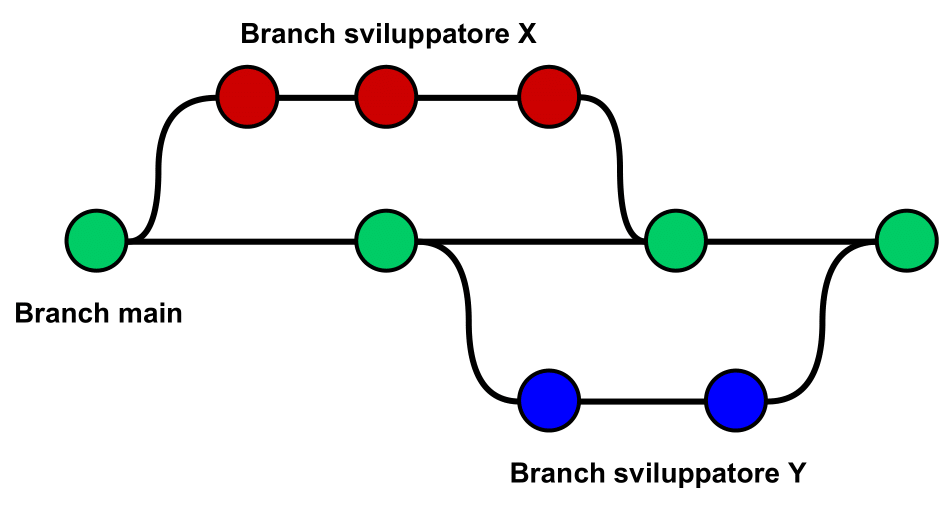
\includegraphics[width=1 \textwidth]{figure/git-branches.png}
    \caption{Rappresentazione grafica del funzioonamento dei branch in Git. Si possono notare i due rami di sviluppo di due programmatori diversi che verranno uniti nel ramo principale.}
    \label{fig:git-branches}
\end{figure}




\section{Docker}
\label{sec:docker}
\textbf{Docker} \`e una piattaforma che gestisce e automatizza la distribuzione di applicazioni tramite l'uso di \textit{container}, in cui vengono inseriti il codice sorgente, le librerie e tutte le dipendenze  necessarie per eseguire il codice, permettendo di rendere eseguibile lo stesso codice su varie macchine in modo affidabile e riproducibile, tramite isolamento dall'architettura su cui viene eseguito. L'isolamento avviene tramite l'uso dei container, che limitano l'accesso dell'applicazione a tutte le risorse del sistema operativo, lasciando  l'accesso solo alle funzionalit\`a necessarie all'esecuzione \cite{ref:docker}. La comodit\`a di utilizzare i container \`e data dalla possibilit\`a di costruire facilmente e velocemente  un ambiente di sviluppo o di test isolato e indipendente dal sistema su cui viene eseguito, garantendo in caso di problemi di effettuare modifiche sulle funzionalit\`a del software.

La creazione e l’inizializzazione  di un'applicazione in un container Docker avviene tramite file chiamati ``immagini''. La stessa immagine pu\`o dar vita a pi\`u container. Ogni immagine \`e definita e creata da un \textbf{Dockerfile}, un file di configurazione contenente tutti i comandi necessari  per assemblare l’immagine. Una immagine pu\`o essere creata  partendo da zero, oppure a partire  da una gi\`a esistente, per esempio scaricandola da Docker Hub\footnote{\url{https://hub.docker.com/}}, sulla quale aggiungere i livelli necessari.
Un file Docker \`e costituito da una serie di comandi formati nel modo seguente: \texttt{ISTRUZIONI   argomenti}, in cui ogni riga rappresenta un livello. Le istruzioni   fornite da Docker, simili a quelle di alcuni linguaggi di programmazione, permettono di svolgere alcune importanti operazioni con lo scopo di creare l'immagine.  Tra queste troviamo l'istruzione \texttt{FROM}, che indica l'immagine di base da cui partire per la creazione di una nuova. Questa istruzione deve essere la prima istruzione nel file Docker. La possibilit\`a di definire variabili è data dall'istruzione \texttt{ARG}; di eseguire comandi durante la fase di compilazione con \texttt{RUN}; di copiare file e directory all'interno dell'immagine con l'istruzione \texttt{ADD}. Si ha inoltre la possibilit\`a di montare directory sul container tramite \texttt{VOLUME}; quando si vuole specificare in fase di esecuzione la porta su cui il container \`e in ascolto  si utilizza \texttt{EXPOSE}. Esistono poi molte altre istruzioni che non  verranno affrontate in questo contesto.



\begin{figure}
    \centering
    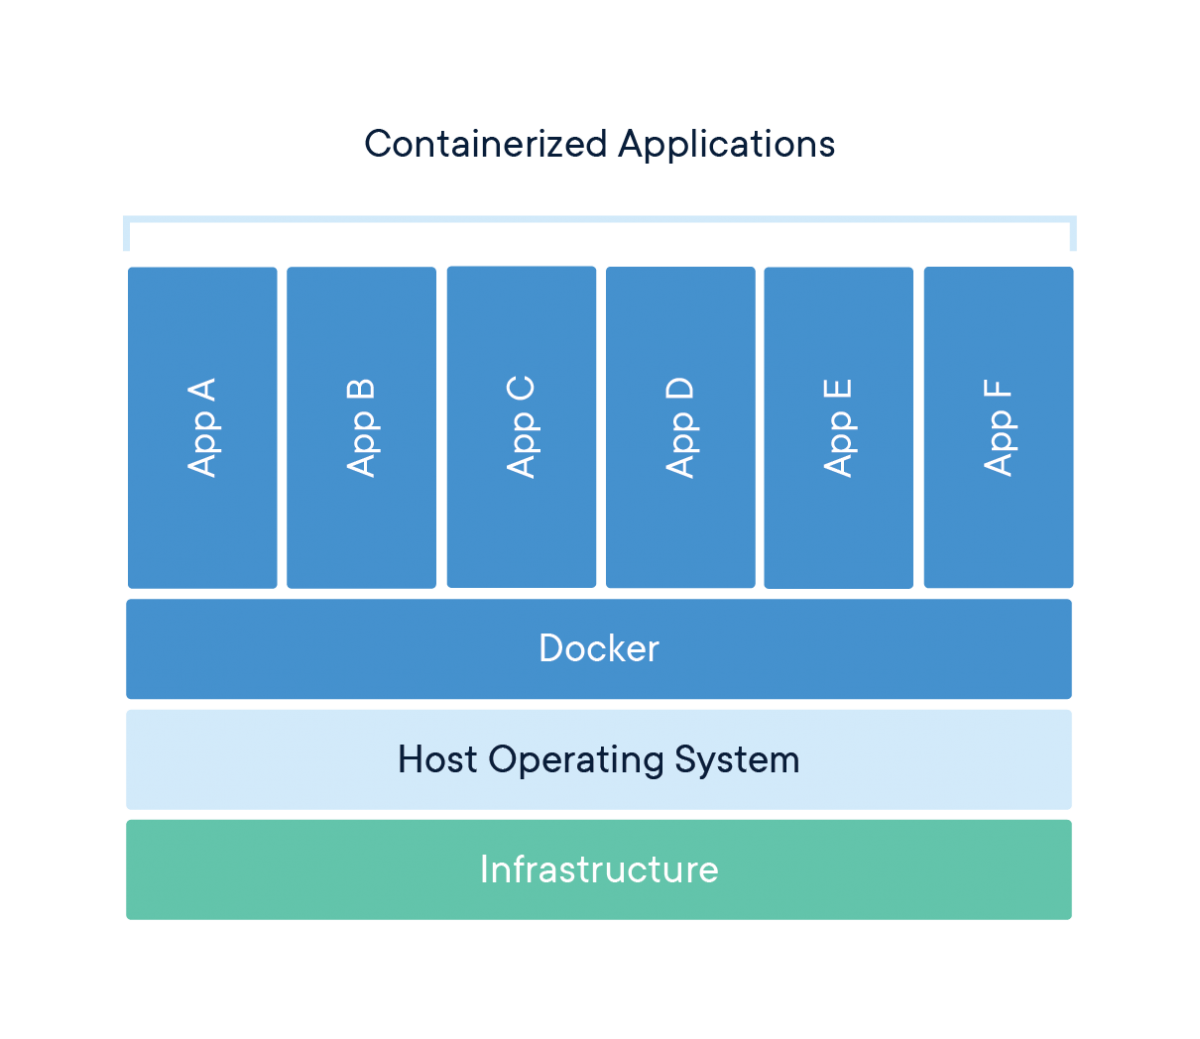
\includegraphics[width=0.5 \textwidth]{figure/docker.png}
    \caption{Astrazione del funzionamento dei container Docker \protect \footnotemark .}
    \label{fig:docker}
\end{figure}

\footnotetext{Immagine presa da: \url{https://www.docker.com/resources/what-container}}

\begin{listing}[H]
\caption{Esempio di Dockerfile \protect \footnotemark.}
\begin{minted}[mathescape,
               linenos,
               numbersep=5pt,
               gobble=0,
               fontsize=\small,
               frame=lines,
               framesep=2mm]{Dockerfile}
FROM golang:1.16-alpine AS build
#Installa le dipendenze necessarie
#Esegue comandi per aggiornare le dipendenze
RUN apt-get update && apt-get install -y 
RUN apk add -no-cache git
RUN go get github.com/golang/dep/cmd/dep
...
#Copia il progetto e lo compila
COPY . /go/src/project/
RUN go build -o /bin/project
...
\end{minted}
\end{listing}

\footnotetext{Fonte: \url{https://docs.docker.com/develop/develop-images/dockerfile_best-practices}}

Grazie a  Docker \`e stato possibile garantire ad ogni sviluppatore di GeneroCity di avere un ambiente di sviluppo con tutto il necessario sul proprio pc in modo semplice.



\section{Postman}
\label{sec:postman}
Postman \`e un software che ha permesso di testare le API in modo facile ed intuitivo. Affronteremo nel dettaglio cosa sono le API e il loro funzionamento nel prossimo capitolo, per ora \`e sufficiente dire che un API \`e software che  mediante  chiamate HTTP (URL) effettua  richieste ad un server, ricevendo indietro una risposta.  Le richieste  possono essere effettuate sia verso un server locale che verso un server online, impostando tutti i dati di una tipica chiamata HTTP,  l'\textit{header},  eventualmente il \textit{body}.  Una volta scelto il metodo della richiesta (per esempio GET, POST...), si inserisce nel apposito campo del programma l'URL che identifica l'API. Dopo essersi eventualmente autenticati, Postman controlla  se i parametri richiesti dalla chiamata (qualora presenti)  sono corretti,  quindi permette di eseguire l'API, e poi restituisce un array di oggetti JSON contenente l'output oppure,  in caso contrario, un errore esplicativo del problema \cite{ref:postman-test}. Dunque Postman permette di effettuare test senza avere l'applicazione, perché permette di valutare in base all'input se viene riportato l'output corretto ed eventualmente di apportare correzioni.



%==================Capitolo 2 background============


\bigskip
\chapter{Background}
\label{cap:cap03}

\section{Che cos'è e come funziona una API}
\label{sec:api}

Prima di parlare del progetto in s\'e,  \`e oppurtuno spiegare nel dettaglio cosa sono le API, poich\'e queste rappresentano un aspetto fondamentale del mio tirocinio.\\

Il termine \textbf{API} (acronimo di  \textit{Application Programming Interface}) indica quel genere di software che offre servizi ad altro software o hardware, tramite un insieme di protocolli e routines volte allo svolgimento di un compito, permettendo una facile comunicazione tra dispositivi diversi. Lo scopo delle API \`e  quello di nascondere i dettagli interni del funzionamento di un sistema, esponendo solo le parti necessarie \cite{ref:api-rh}. Le API semplificano il design e l’architettura dei software, aggiungono flessibilit\`a e sicurezza, e permettono scalabilit\`a e manutenzione nel tempo.
In una API agiscono due attori:
\begin{itemize}
    \item \textbf{Client:} colui che effettua la chiamata per ottenere i dati. Non \`e necessario che conosca il funzionamento del programma sottostante il server, basta solo che sia a conoscenza delle regole necessarie per implementare la chiamata.
    \item \textbf{Server:} l'elemento che su richiesta fornisce i dati corrispondenti alla chiamata ricevuta gestendo e implementando le regole di funzionamento dell’API.
\end{itemize}


%Sono formate da definizioni e protocolli con i quali vengono realizzati e integrati software applicativi. Lo scopo di un API è quello di ottenere porsi tra l'hardware ed il software. Nel caso di un applicaizone mobile come GeneroCity un APi si frappone tra la parte di frontend (quella visibile all'utente) e il databse, difatti permette a chi usa l'app di svolgere alcuen funzioni (spesso sono chiamate su databse). Un'API è spesso composta da diverse parti che fungono da strumenti o servizi a disposizione del programmatore.


%Una buona API fornisce una "scatola nera", cioè un livello di astrazione che permette al programmatore di evitare di conoscere il funzionamento delle API ad un livello più basso. Questo permette di riprogettare o migliorare le funzioni all'interno dell'API senza cambiare il codice che si affida ad essa. 

Le API consentono l'accesso alle risorse mantenendo \textbf{sicurezza} e \textbf{controllo}, in quanto \`e il programmatore a decidere come e a chi concedere l'accesso. Alcuni esempi di API sono le librerie usate nei linguaggi di programmazione,  oppure quelle che consentono ad uno sviluppatore software di accedere a determinate parti di un sistema operativo senza necessariamente conoscerne il funzionamento a basso livello.
Le API pi\`u utilizzate sono quelle che  sfruttano come canale di comunicazione  Internet. Queste ultime utilizzano in genere il protocollo HTTP (acronimo di \textit{HyperText Transfer Protocol}, presentato nella prossima sezione) per mettere in comunicazione i vari elementi. I messaggi di risposta di queste API sono in genere sotto forma di file JSON \footnote{Questo genere di file \`e lo standard di fatto quando si vuole scambiare dati tra client e server. Sono formati da array di valori sotto forma di \texttt{chiave:valore}}, in modo da consentire ad altre app una gestione dei dati pi\`u facile.
Le principali politiche di rilascio di un'API sono le private,  o le pubbliche. Con  le private l'API \`e solo per uso ristretto, interno dell'azienda. Con un rilascio pubblico, le aziende   consentono  invece agli sviluppatori di terze parti riconosciuti di accedere alle API. Se l'API \`e disponibile per l'utilizzo da parte del pubblico spesso l'accesso pu\`o essere ristretto utilizzando ``token API'' o convalide del cliente.\\

\subsection{Messaggi HTTP}
HTTP \`e un protocollo a livello applicativo di tipo client-server, usato principalmente in ambito web. Le comunicazioni tra client e server vengono effettuate tramite messaggi HTTP. I messaggi di richiesta sono costituiti da una \textbf{riga di richiesta} (conosciuta anche con il nome di \textit{request-line}) composta da un metodo, una URL e versione del protocollo, una intestazione detta \textbf{header}, che contiene metadati inerenti l'host e il client; e da un corpo, \textbf{body}, che contiene  le informazioni che si vogliono trasmettere \cite{{ref:http-protocol}}.  Ogni richiesta ha nella sua request-line un determinato metodo HTTP. I metodi comunicano al server cosa fare con i dati identificati dalla URL. Quelli maggiormente usati nello sviluppo di API sono GET, POST, PUT e DELETE. 

\begin{description}
    \item \textbf{GET} Ordina al server di trasmettere al client le informazioni identificate nella URL, le informazioni lato server non vengono modificate in questo tipo di richiesta. 
    \item \textbf{PUT} Usata quando si vuole creare o aggiornare la risorsa identificata dalla URL. Per esempio, la chiamata
    \texttt{PUT /users/user1}     crea un utente di nome user1. Nella richiesta non c'\`e alcuna indicazione che indichi  al server come vadano creati i dati ma solo che deve farlo: queste informazioni risiedono nel corpo della richiesta.
    \item \textbf{DELETE} Opera inversamente al PUT, viene usato quando si vuole cancellare la risorsa identificata dalla URL. Per esempio, \texttt{DELETE /users/user1}
    elimina tutte le informazioni associate alla risorsa identificata da \texttt{/users/user1}.
    \item  \textbf{POST} Utile  quando si vuole inviare grandi quantit\`a di dati, come un file o un'immagine al server.
 \end{description}

%La risposta HTTP deve specificare il tipo di contenuto del corpo. Questo deve essere fatto nell'intestazione, nel campo \texttt{Content-Type} ad esempio: \texttt{Content/Type: application/json}.

I messaggi di risposta, sono invece formati da una \textbf{riga di stato}, un \textbf{header}, che indica  il tipo e la versione del server ed il tipo di contenuto restituito, e da un \textbf{body} contenente il contenuto restituito. Generalmente  nelle API il contenuto viene riportato sotto forma di JSON o XML. Le risposte vengono inoltre affiancate  da \textbf{codici di stato} che indicano l'esito della richiesta. Il server dovrebbe restituire il codice di riposta pi\`u appropriato, in modo da far capire al client il problema che si \`e presentato ed eventualmente rimediare agli errori. La \autoref{tab:codici-http} riporta i codici maggiormente usati.

\begin{center}
\begin{table}[H]
    \center
    \caption{Codici di stato HTTP.}
    \label{tab:codici-http}
    \begin{tabular}{|c c|}
    \hline
     \textbf{Codice} & \textbf{Significato}   \\  
        \hline
       
        200 & OK. Richiesta valida e andata a buon fine.   \\
        \hline
        
        201 & Creato. Richiesta valida, la risorsa \`e stata creata.  \\  
        \hline
        
        400 & Non valida. La richiesta non \`e stata formata in modo corretto.   \\
        \hline
       
        401 & Non autorizzato. Si richiede l'autenticazione prima di accedere alla risorsa.   \\
        \hline

        403 & Proibito. Utente autenticato ma non possiede il permesso necessario. \\
        \hline

        404 & Non trovato. La risorsa richiesta non pu\`o essere raggiunta.   \\
        \hline

        500 & Errore interno al server. Processo fallito lato server, in circostanze impreviste.    \\ 
        \hline

    \end{tabular}
\end{table}
\end{center}

% \begin{center}
% \begin{figure}[H]
%     \centering
%     \includegraphics[width=0.8 \textwidth]{figure/api.png}
%     \caption{Funzionamento API. DA SOSTITUIRE}
% \end{figure}
% \end{center}


\begin{center}
\begin{figure}[H]
    \centering
    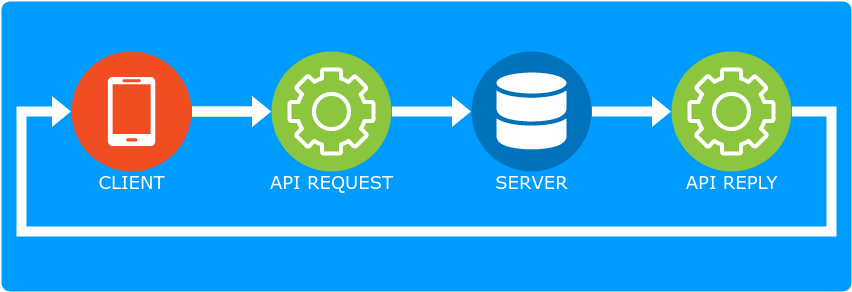
\includegraphics[width=1 \textwidth]{figure/api2.png}
    \caption{Schema di funzionamento di una API. Il client fa una richiesta tramite API, l'API interagisce con il DB e restituisce una risposta.}
\end{figure}
\end{center}



%Generazione di una richiesta o chiamata all’API per recuperare le informazioni.
%L'API effettua a sua volta una chiamata al programma esterno o al server web.
%Il server invia una risposta all'API con le informazioni richieste.
%L'API trasferisce i dati all'applicazione richiedente iniziale.




\section{Struttura back-end dell'app GeneroCity}

In questo paragrafo vedremo come le tecniche generali precedentemente presentate sono state usate nell'applicazione GeneroCity. Ricordiamo che un'applicazione \`e formata da una parte  di \textbf{font-end} e da una parte  di \textbf{back-end}, in comunicazione: il front-end  \`e la parte di interfaccia grafica con cui interagisce l'utente, \`e la parte visibile,  serve ad acquisire o presentare   dati  all'utente. La parte  di \textbf{back-end}, non visibile all'utente,  riceve le chiamate dal front-end, e si occupa di implementare tutto il funzionamento e la logica dell'applicazione e di elaborare i dati ricevuti. Il mio lavoro di tirocinio si concentra sulla parte back-end, spiegata brevemente nel seguito.\\

Il back-end è costituito da file e cartelle. Ci sono i file di configurazione, il Dockerfile (\autoref{sec:docker}), il file con la collezione delle API da importare in Postman (\autoref{sec:postman}), quelli utili all'esecuzione del progetto. Le cartelle principali  che si occupano di far funzionare l'applicazione sono: la cartella \texttt{cmd/} che ha lo scopo di costruire e gestire tutte le strutture necessarie al funzionamento dell'applicazione, essa  contiene anche l'eseguibile principale, la cartella \texttt{database/} predisposta alla creazione e modifica del database e la cartella \texttt{service/} che contiene tutti i file per il funzionamento delle  API. Grazie alla modularit\`a garantita dai packages Go, ogni directory contiene tutti i file  predisposti allo svolgimento di un singolo compito.


\subsection{Inizializzazione dell'app}
La cartella \texttt{cmd/}  si occupa di gestire tutti gli strumenti per la fase di inizializzazione e di ``costruzione'' del progetto partendo dall'eseguibile principale (il \texttt{main}). 
Un file di questo package contiene la configurazione dell'applicazione, ovvero la struttura che compone l'applicazione con tutte le dipendenze necessarie. 
\\
Il \texttt{main}   carica  la configurazione ed inizializza  le variabili globali, poi  costruisce l'applicazione effettiva, assemblando e inizalizzando tutte le componenti e effettuando i dovuti controlli sulla loro corretta costruzione  e sul loro stato. Tra le componenti utili all'applicazione ci sono: la cache, utile a  velocizzare la comunicazione, il server web, per la comunicazione tra i componenti, il servizio di autenticazione, il log degli errori (in cui vengono salvati eventuali errori di esecuzione), il gestore delle notifche, il database ed altri.


\subsection{Database}
Il package \texttt{database/} mantiene tutti i file utili per la creazione e l'aggiornamento del database dell'applicazione. In particolare \`e presente un file con la copia attuale dello schema del database (ovvero struttura delle varie tabelle ed i collegamenti tra esse), e i file predisposti alle migrazioni. I file di migrazione dello schema sono quei file che, mediante l'ausilio di alcuni strumenti, permettono di aggiornare o ripristinare in automatico versioni e modifiche fatte ad un database (es. aggiunta o rimozione di tabelle e colonne) gi\`a in utilizzo, permettendo di addattare i dati al cambiamento dei requisiti in maniera sicura. Nel nostro caso, tra le tabelle pi\`u importanti ci sono quella predisposta a mantenere informaizoni sugli utenti, quella che mantiene le informazioni sulle auto, quella per i parcheggi (coordinate, l'orario, utente e auto che ha effettuato il parcheggio...) e quelle con la storia dei match tra gli utenti, ovvero i dati che associano i vari utenti (con le rispettive automobili) che hanno scambiato un parcheggio.


\subsection{Gestione delle API}

Il package \texttt{service/} rappresenta il punto di ingresso dell'applicazione. 
Esso implementa all'interno della funzione \texttt{New()} un router (costruito utilizzando una libreria di Go, che implementa una comunicazione HTTP tra un client ed un server) interno, ovvero quella componente che farà da ``ricevitore'' dell'applicazione confrontando le richieste in entrata e chiamando un gestore per gli URL, presenti nell'\textbf{handler}. L'handler è il file che si occupa di mappare tutte le funzioni che implementano le API con l'URL per le chiamate, dunque si occupa di una delle operazioni più importanti per GeneroCity. 
Nel package \texttt{service/} sono presenti inoltre tutti i file che implementano la logica delle API, le strutture che dovranno essere restituite come output ed infine i file che permettono l'interazione delle API con il database. Infatti ogni API di GeneroCity è composta di due parti: il file principale che svolge la funzione di ricevere i dati in input, fare i controlli necessari e dare il corretto output, con annesso codice di stato, ed una parte che si occupa di interagire con il database mediante comandi SQL, chiamato dal file principale. Queste due parti sono tenute separate per fornire maggiore flessibilità ai cambiamenti in futuro. Tra le API che hanno un ruolo fondamentale ci sono:

\begin{description}
    \item  \textbf{createMe} Si occupa di creare un utente nel sistema, inizializzare tutti i dati ad esso associati ed assegnargli un identificativo univoco (quest'ultimo utile per effettuare query sul database), prende dal body il nickname da assegnare all'utente.
    \item  \textbf{createCar} Prende in input dal body vari dati, come targa, nome, dimensioni, modello e colore dell'auto, e crea un ``oggetto'' \textit{auto} associato ad uno o più utenti (per esempio ad utenti nella stessa famiglia).
    \item \textbf{parkCar} Una volta passato nel path dell'API l'identificativo dell'auto e nel body le coordinate geografiche del parcheggio, il momento del parcheggio ed il viaggio effettuato (un array  JSON che mantiene informazioni su ogni coordinata del viaggio effettuato per arrivare a quel parcheggio), se i controlli su tali dati sono andati a buon fine,  aggiorna lo stato dell'auto in ``parcheggiata'' e aggiunge una nuova riga nella tabella dei parcheggi.
    \item \textbf{unparkCar}  Opera in maniera opposta alla precedente e aggiorna lo stato dell'automobile  da ``parcheggiata'' a ``non parcheggiata''.
    \item \textbf{createMeGiver} Serve per effettuare lo scambio di parcheggio, segnalando al sistema (e agli altri utenti) il luogo e il momento in cui l'utente lascia il parcheggio.
    \item \textbf{createMeTaker} Complementare alla precedente, indica al sistema (e agli altri utenti) che l'utente cerca parcheggio in una determinata area, indicata dalle coordinate geografiche inserite nel body della richiesta.
    \item \textbf{createChatMessage} Permette di mandare un messaggio ad un altro utente, il testo viene passato nel body.
    \item \textbf{getParkList} Selezionando un intervallo di tempo e ritorna un array con tutti i parcheggi effettuati in quell'intervallo, con informazioni come inizio e fine del parcheggio, via e auto con cui si \`e fatto il parcheggio.
    \item \textbf{getFamily} Restituisce l'elenco di tutti gli utenti che hanno accesso all'automobile selezionata.
\end{description}

Sono poi presenti altre API che permettono all'utente di visualizzare, modificare o eliminare dati.

%https://bmwtraderonline.info/hay-south/what-is-application-programming-interface-api.php


\section{Lavoro svolto}

Il percorso che ho fatto in questi mesi mi ha permesso di avvicinarmi, per quanto   possibile in sede di un tirocinio universitario,  con quella che in ingegneria del software viene definita \textbf{metodologia agile}, ovvero una serie di tecniche  che puntano allo sviluppo di software che sia focalizzato sull'obiettivo di consegna, in tempi brevi e frequenti (\textit{early delivery}), e sia funzionante e di qualit\`a. Infatti, settimanalmente venivano svolte riunioni con il professore ed il team volte a fare il punto della situazione e a progettare il lavoro per la settimana successiva, promuovendo quindi lo sviluppo iterativo ed incrementale del progetto e l'organizzazione autonoma del lavoro. Ho imparato a seguire una pianificazione a breve termine che gestisce l'andamento del progetto, tenendo anche conto di eventuali  cambiamenti in corso d'opera. \\   


Dopo un periodo di apprendimento e di studio del progetto, che era gi\`a in fase di sviluppo quando ho cominciato il tirocinio, nel quale ho dovuto capire il funzionamento e le tecnologie utilizzate, mi \`e stato assegnato il primo dei miei due compiti: l'aggiornamento del codice, e lo sviluppo delle API.


\subsection{Aggiornamento struttura del codice}

Poiché l'applicazione era gi\`a stata avviata tempo prima, sorgeva la necessit\`a di un aggiornamento e di alcune modifiche che garantissero una scalabilit\`a maggiore del progetto in futuro. In particolare mi sono occupato di:
\begin{itemize}
    \item \textbf{Modifica di librerie:} ho dovuto modificare quei metodi che usano versioni vecchie di librerie, cercando di adattarli quando possibile alla nuova versione, altrimenti usando una libreria alternativa che potesse svolgere lo stesso compito.
    \item \textbf{Riprogettazione file di configurazione:} era necessario riposizionare il codice presente nel main che rappresentava i vari elementi utili al progetto (database, server...) in file di configurazione appositi, riprogettando le chiamate e gli usi di essi, per favorire la suddivisione del codice in base alle funzioni svolte.
    \item \textbf{Adattamento delle API:} ho dovuto riallineare le API pre-esistenti alle modifiche della nuova versione.
    \item \textbf{Riscrittura routine autenticazione:} a seguito di alcuni cambiamenti \`e risultato necessario   riscrivere la routine che si occupa del token di autenticazione per il software di testing delle API. 
    \item \textbf{Individuazione di bug:} segnalare e possibilmente risolvere alcuni piccoli bug emersi durante il lavoro. 
\end{itemize}

Il compito che mi \`e stato affidato  si \`e rivelato inizialmente ostico, ha dunque  richiesto del tempo  per capire come operare. Inoltre mi sono trovato davanti ad problemi inaspettati, che mi hanno richiesto di  capire da dove fossero generati e come risolverli. Grazie anche alla collaborazione con  altri colleghi del team, il lavoro preparatorio mi ha permesso di prendere confidenza con il codice,  con le modalit\`a e i tempi di gestione di un progetto del genere.

\subsection{Progettazione delle API}
\label{sec:prog-api}

L'altro compito che mi è stato assegnato \`e quello di progettare e sviluppare delle specifiche API per GeneroCity. L'intento era quello di fornire dati che evidenziassero all'utente i vantaggi derivanti dall'uso di GeneroCity, ovvero quello ottimizzare i tempi e minimizzare il percorso per il parcheggio.

La prima cosa che ho dovuto fare insieme ad un collega che si occupa della parte di front-end  \`e ragionare  mediante \textbf{need-finding}\footnote{Il need-finding \`e un insieme di tecniche prevalentemente basate su domande e questionari, da somministrare ai possibili utenti finali di un'applicazione, che aiutano nella fase di progettazione delle funzionalità, poich\'e permettono di immaginare cosa realmente interessa all'utente, indirizzando cos\`i lo sviluppo nella corretta direzione, risparmiando risorse ed evitando lo sviluppo di funzionalit\`a non usate.}
e sondaggi, su quali dati potessero essere utili allo sviluppo. L'idea di base che \`e emersa, considerando anche lo stato attuale dell'applicazione, \`e quella di evidenziare la distanza percorsa ed il tempo impiegato dall'utente ad effettuare parcheggi. 

Inizialmente l'idea era quella di rappresentare dati solamente inerenti  all'utente, ma durante le riunioni settimanali  raffinando i requisiti \`e emerso che potesse essere utile avere dati anche riguardo alle auto, in quanto queste possono essere usate da vari membri della famiglia che usano l'applicazione.  
I dati di interesse inerenti alle statistiche di ricerca dell'utente, che verranno quindi inseriti nel database dell'applicazione sono:
\begin{itemize}
\item \textbf{Tempo totale:} ovvero il tempo totale in secondi impiegato dall'utente per effettuare i parcheggi.
\item \textbf{Distanza totale:} la distanza totale in chilometri impiegata dall'utente per cercare parcheggio.
\item \textbf{Media tempo di ricerca:} media totale in secondi del tempo impiegato a cercare parcheggio, indica all'utente quanto tempo impiega mediamente (e quindi indirettamente quanto ne risparmia) nella ricerca di parcheggio.
\item \textbf{Media distanza di ricerca:} media totale in chilometri della distanza percorsa dall'utente  a cercare parcheggio.
\item \textbf{Numero di match:} ovvero il numero di parcheggi che l'utente ha trovato usando la funzionalit\`a di scambio parcheggio dell'applicazione.
\item \textbf{Numero parcheggi senza match:} numero di parcheggi che l'utente ha trovato senza usare la funzione di scambio. 
\item \textbf{Numero di parcheggi:} numero totale dei parcheggi effettuati.  
\end{itemize}

I dati di interesse inerenti alle auto sono:
\begin{itemize}
    \item \textbf{Tempo totale:}  il tempo totale, in secondi, di ricerca dei parcheggi svolti con una stessa auto.
    \item \textbf{Media tempo:} tempo medio, in secondi, impiegato a ricercare parcheggio.
    \item \textbf{Distanza totale:} chilometri percorsi dall'auto a cercare parcheggio.
    \item \textbf{Distanza media:}   media dei chilometri percorsi da un'auto per cercare parcheggio.
    \item \textbf{Numero di match:} ovvero il numero di parcheggi fatti con la stessa auto  usando la funzionalit\`a di scambio parcheggio dell'applicazione.
    \item \textbf{Numero parcheggi senza match:} numero di parcheggi fatti con la stessa auto  senza usare la funzione di scambio. 
    \item \textbf{Numero parcheggi:}  il numero totale di parcheggi fatti da qualsiasi utente con la stessa auto. 
\end{itemize}

% \begin{center}
% \begin{table}[H]
%  %    \caption{Rappresentazione dei dati statistci sul l'utente.}
% \label{tab:statistiche-utente}
% \begin{tabularx}{\textwidth}{l  X}

%     \hline
%     \textbf{Campo} & \textbf{Significato} \\  
%     \hline
%     userId  & Rappresenta l'ID dell'utente interessato, utile per effettuare le query. \\
%    \hline
%     totaltimesearching   &  Tempo totale, in secondi, in cui l'utente ha cercato parcheggio. \\  
%    \hline
%     totaldistance & Distanza totale, in secondi, percorsa dall'utente cercando aprcheggio. \\      
%    \hline
%     avgtimesearching  & Media totale, in secondi, del tempo impiegato a cercare parcheggio. \\
%     \hline
%     avgdistance   & Media totale, in chilometri,  della distanza percorsa a cercare parcheggio. \\
%     \hline 
%     matchnumber  &  Numero totale di parcheggi trovati usando la funzione di scambio. \\
%  \hline   
%     searchingtimematch  & Tempo totale, in secondi, in cui l'utente ha cercato parcheggio usando la funzione di scmabio. \\
%     \hline   
%     matchdistance   & Distanza totale, in chilometri, in cui l'utente ha cercato parcheggio usando la funzione di scmabio. \\
%     \hline  
%      avgmatchdistance & Media, in chilometri,  della distanza percorsa a cercare parcheggio usando la funzione di scmabio. \\
%     \hline 
%       avgtimematch   & Media, in secondi,  del tempo impiegato a cercare parcheggio usando la funzione di scmabio. \\
%        \hline   
%     nomatchnumber  & Numero di parcheggi effettuati senza utilizzare la funzione di scmabio. \\
%        \hline 
%       searchingtimenomatch  & Tempo totale, in secondi, in cui l'utente ha cercato parcheggio senza usare la funzione di scmabio parcheggio. \\
%        \hline  
%      avgtimenomatch  & Media, in secondi,  del tempo impiegato a cercare parcheggio senza usare la funzione di scmabio. \\
%        \hline 
%       avgnomatchdistance  & Media, in chilometri,  della distanza percorsa a cercare parcheggio senza usare la funzione di scmabio. \\
%       \hline
% \end{tabularx}
%  \end{table}
%  \end{center}


%\begin{center}
%\begin{table}[H]
%    \caption{Rappresentazione dei dati statistci sulle auto.}
%\label{tab:statistiche-auto}
%\begin{tabularx}{\textwidth}{l X}
%       \hline
%    \textbf{Campo} & \textbf{Significato} \\  
%    \hline
%    cid & ID dell'auto interessata.\\
%    \hline
%    parknumber & Numero parcheggi di  fatti con l'auto. \\
%    \hline
%    totalcartime & Tempo totale, in secondi, di ricerca dei parcheggi svolti con l'auto.\\
%    \hline
%    avgcartime & Tempo medio, in secondi, di ricerca dei parcheggi.\\
%    \hline 
%    totalcardistance & Distanza totale, in chilometri, percorsa dall'auto a cercare parcheggio.\\
%    \hline
%    avgcardistance &  Distanza media percorsa dall'auto per cercare parcheggio.\\
%         \hline
%\end{tabularx}
% \end{table}
 %\end{center}

Con questi dati chi si occupa di progettare la parte dell’interfaccia dell’applicazione ha la possibilit\`a di presentare all’utente quanto tempo imipega nella fase di parcheggio, permettendo ad esso di prendere coscienza di tali informzioni ed invogliandolo sempre di pi\`u all'utilizzo dell'applicazione come strumento di supporto nell'impiego di tempo in maniera efficente. 
\\

L'idea per arrivare a ottenere questi dati \`e la seguente: dopo che si \`e calcolato i dati del tempo di ricerca e distanza di ricerca, associati ad ogni parcheggio, si effettuano i calcoli e si salvano nel database tramite un API che effettua la \texttt{PUT}, in modo di evitare di ripetere il calcolo  ad ogni chiamata delle API che effettuano la \texttt{GET} aumentando l'efficienza.
\\

Lo schema di progettazione del funzionamento dell'API per le statistiche sull'utente è mostrata nella \autoref{fig:statistiche-utente}. Come prima cosa si controlla che l'id dell'utente sia corretto, sebbene  è raro che si verifichi un tale errore. Se il controllo non va a buon fine si ritorna il codice di stato 400, con spiegazione dell'errore associato. Altrimenti si può proseguire con la funzione che interagisce con il database, se le query vengono effettuate correttamente si ritornano i dati statistici. Quando l'interazione col database non va a buon fine le cause possono essere due: l'id dell'utente non è presente nella tabella, allora ritorna il codice 404 che indica che la risorsa non è stata trovata; oppure può accadere che il database non sia raggiungibile e quindi ritorna codice di stato 500.

\begin{center}
\begin{figure}[H]
    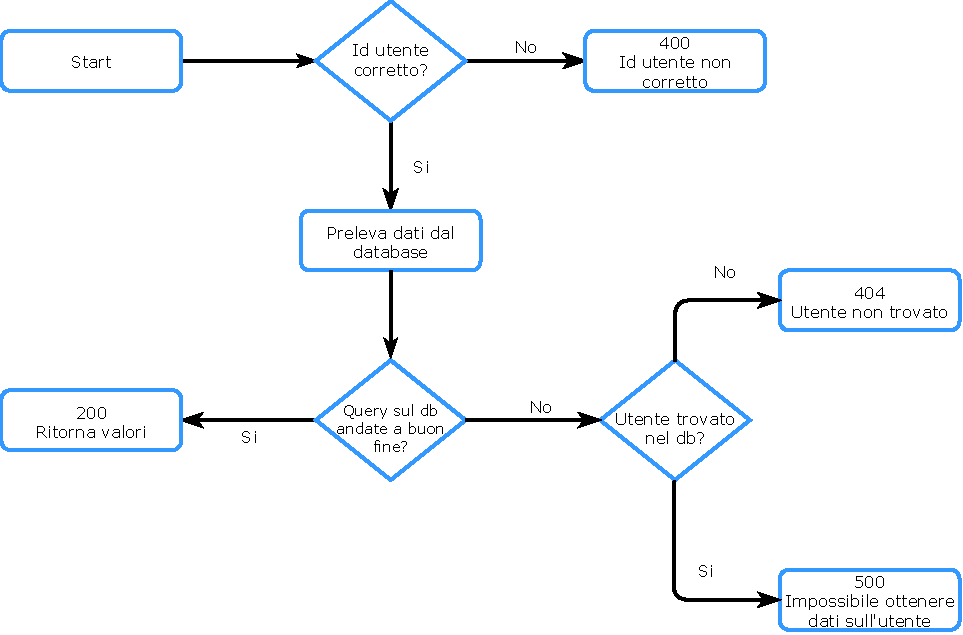
\includegraphics[width=\textwidth]{figure/user-statistics-flow-chart.pdf}
    \caption{Funzionamento API per ottenimento delle statistiche sull'utente.}
    \label{fig:statistiche-utente}
\end{figure}
\end{center}


La \autoref{fig:statistiche-auto} rappresenta l'idea dietro l'API  per l'ottenimento delle statistche sull'auto. Viene inizialmente controllata la correttezza dell'id dell'auto, se il controllo va a buon fine si verifica che l'utente che ha effettuato la chiamata all'API sia associato all'auto di interesse, se non lo è ritorna il codice 403 (l'utente non è autorizzato all'accesso alla risorsa). Altrimenti si possono effettuare le query sul database, se non raggiungibile ritorna codice 500 se invece non si trova l'id dell'utente allora ritorna 404, negli altri casi in cui le query vanno a buon fine e si restituisce il codice di stato 200.

\begin{center}
\begin{figure}[H]
    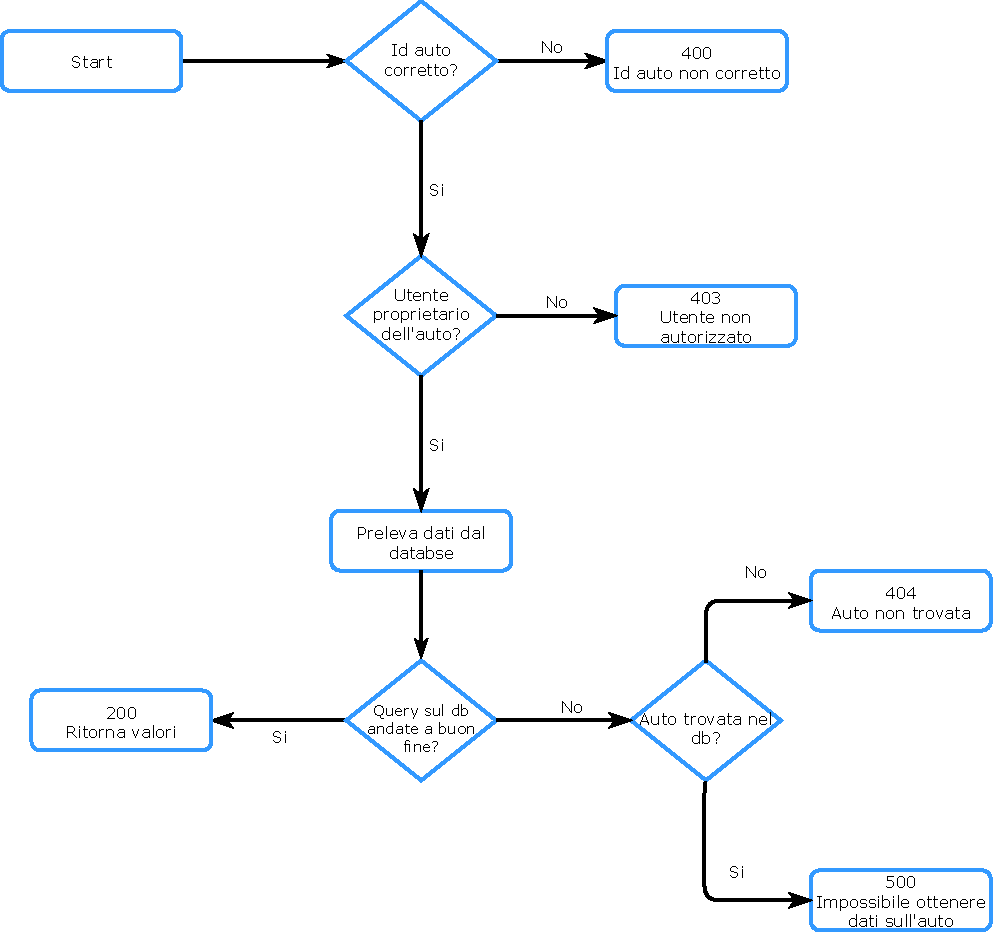
\includegraphics[width=\textwidth]{figure/car-statistics-flow-chart.pdf}
    \caption{Funzionamento API per ottenimento delle statistiche sull'auto.}
    \label{fig:statistiche-auto}
\end{figure}
\end{center}


% \begin{itemize}
%     \item ID utente, di tipo stringa, rappresenta l'ID dell'utente interessato utile inotlre per effettuare le query.
%     \item Tempo totale di ricerca, che verrà rappresentato come un intero e rappresenta il tempo totale, in secondi, in cui l'utente ha cercato parcheggio.
%     \item  Media tempo di ricerca, rappresentato da un tipo float, media totale, in secondi, del tempo impiegato a cercare parcheggio.
%     \item  Media distanza di ricerca, tipo float, indica la media totale, in chilometri,  della distanza percorsa dlal'utente a cercare parcheggio.
%     \item Numero di match, intero, numero totale di parcheggi trovati usando la funzione di scambio parcheggio
% \end{itemize}

%============Capitolo 3 implementaizone========

\bigskip

\chapter{Implementazione API}
\label{cap:cap04}

In questo capito presento la parte di sviluppo in linguaggio Go mediante anche l'ausilio di alcune parti di codice.

\section{Estrapolazione dei dati tramite l'API car park}

Come prima cosa per ogni parcheggio vanno associati i valori inerenti al tempo di ricerca e la distanza percorsa, tramite i quali si estrapoleranno tutte le altre statistiche. Nel sistema per parcheggio non si intende solamente il luogo fisico, ma un oggetto che contiene le informazioni sul viaggio, sullo stato dell'auto e sul momento e luogo effettivo del parcheggio.

Successivamente, prendendo in cosiderazione l'intero viaggio dell'auto da un parcheggio all'altro, estrapolo solo i dati inerenti la fase di ricerca. Per fare questo ho ampliato una API già esistente, \textbf{car-park}. Questa API prende in input dal body anche un campo \textbf{tripjson}, ovvero una stringa con struttura di un file JSON, che rappresenta il viaggio dell'auto, sotto forma di coordinate geografiche, da un parcheggio all'altro. Proprio il \textbf{tripjson} rappresenta il punto di partenza di tutto lo sviluppo, questo campo è un insieme di posizioni, detti \textbf{tripoint}, formati come  segue:


\begin{listing}[H]
\caption{Esempio di un dato in tripjson.}
\begin{minted}[linenos,
               numbersep=5pt,
               gobble=0,
               fontsize=\small,
               frame=lines,
               framesep=2mm,
               breaklines]{json}
  {
    "speed" : 21,
    "searching" : 0,
    "lat" : 41.9018889,
    "lon" : 12.511498,
    "date" : "2021-10-28T13:24:58+02:00"
  }
\end{minted}
\end{listing}

Di seguito la spiegazione dei vari valori:
\begin{itemize}
	\item Il campo \textbf{speed} indica la velocità dell'auto in quel momento.
	\item \textbf{Searching} indica se l'auto è in fase di parcheggio, quando vale 0 allora l'auto non sta cercando parcheggio. La fase di ricerca viene  attivata o tramite deduzione di un modello di machine learning (in questo caso sarà presente nei tripoint anche un campo denominato ``falsepositive''), o tramite indicazione esplicita dell'utente.
	\item I due valori \textbf{lat} e \textbf{lon} indicano le coordinate geografiche in quell'istante.
	\item Il campo \textbf{date} rappresenta il momento della cattura dei dati. 
\end{itemize}


Quindi l'idea è quella di scorrere l'intero JSON del viaggio individuando il primo punto in cui comincia la ricerca di parcheggio (quello che ha valore \textbf{searching} maggiore di 0), da questo punto in poi calcolare la distanza temporale e spaziale di un punto dal punto precedente. Dopo aver effettuato le somme delle distanze, queste vengono associate al parcheggio di riferimento. Il tutto è mostrato nella seguente parte di codice:


\begin{listing}[H]
\caption{Codice di carPark per il calcolo dei tempi e distanze di ricerca.}
\begin{minted}[linenos,
               numbersep=5pt,
               gobble=0,
               fontsize=\small,
               frame=lines,
               framesep=2mm,
               breaklines]{go}
err = json.Unmarshal([]byte(carPark.TripJson), &data)
...               
var startSearching bool
var searchingDist float64
var searchingTime int
for i := 0; i < len(data)-1; i++ {
	if data[i].Searching > 0 {
		startSearching = true
	}
	if data[i].FalsePositive {
		startSearching = false
	}
	if startSearching {
	  searchingDist += locationutils.HaversineDistance ((data[i+1].Lat),(data[i+1].Lon), (data[i].Lat),(data[i].Lon))
	  diff := data[i+1].Date.Sub(data[i].Date)
	  searchingTime = searchingTime + int(diff.Seconds())
  }
}
carPark.SearchingDistance = searchingDist
carPark.SearchingTime = searchingTime
...
\end{minted}
\end{listing}

Nel dettaglio il funzionamento è il seguente. Prima si converte la stringa \texttt{tripJson} passata dal body (\texttt{carPark.Tripstrut}, rappresenta il valore tripjson preso dla body dell'API) in un oggetto iterabile in Go, chiamato \texttt{data}, usando il metodo \texttt{Unmarshal} della libreria ``encoding/json''  \cite{ref:encoding-json}. Dopo aver fatto opportuni controlli (per esempio che i vari dati esistano e che siano corretti), si effettua l'algoritmo visto nel codice. 

 Si creano le due variabili per la distanza e il tempo, e quella booleana, inizializzata a \texttt{false}, che indica se la ricerca è iniziata. Si itera poi sulla struct\footnote{Una struct è un tipo definito dal programmatore che rappresenta una raccolta di campi, quando si ritiene opportuno cha tali campi vadano raggruppati in un unico elemento anziché essere tenuti separati.} che rappresenta tutto il trip. Se il punto su cui si sta iterando ha il campo ``searching'' maggiore di 0, si mette a \texttt{true} la variabile \texttt{startSearching}. Il secondo controllo serve per evitare i falsi positivi; infatti se nel trip è presente il campo ``falsepositive'', allora vuol dire che c'è stato un errore nella rilevazione automatica. Quindi, se la variabile \texttt{startSearching}  è \texttt{true}, si calcola la distanza delle coordinate tra gli ultimi due punti, usando il metodo della libreria che implementa la formula di Haversine \cite{ref:hv-formula}. Tale formula calcola la distanza in chilometri tra due punti geografici, date  la longitudine e  la latidudine.  Tale distanza viene poi sommata a quella già calcolata in precedenza. Si effettua anche il calcolo  per il  tempo, in secondi. Infine le ultime due righe del codice associano i valori   alla struct \texttt{CarPark}.
Quest'ultima viene quindi passata alla funzione che interagisce con il databse per effettuare l'aggiornamento dei dati appena calcolati.\\


Illustriamo ora la parte di codice predisposta al calcolo degli altri dati.
\begin{listing}[H]
\caption{Codice per il calcolo dei dati in \texttt{CarPark}.}
\begin{minted}[linenos,
               numbersep=5pt,
               gobble=0,
               fontsize=\small,
               frame=lines,
               framesep=2mm,
               breaklines]{go}
...
err = tx.Get(&stat, "SELECT SUM(searchingtimesec) AS totaltimesearching, SUM(searchingdistance) AS totaldistance, AVG(searchingtimesec) AS avgtimesearching, AVG(searchingdistance) AS avgdistance FROM parks WHERE usedby = ?  AND parkstatus = 'park' AND searchingtimesec > 0", userId.String())
if err != nil {
	_ = tx.Rollback()
	return nil, errors.Wrap(err, "select1 statement")
}

err = tx.Get(&stat, "SELECT COUNT(*) AS parknumber FROM parks WHERE parkstatus = 'park' AND usedby = ?", userId.String())
if err != nil {
	_ = tx.Rollback()
	return nil, errors.Wrap(err, "select2 statement")
}

err = tx.Get(&stat, "SELECT COUNT(*) AS matchnumber FROM matches_history WHERE takerid = ? AND status = 'success' ", userId.String())
if err != nil {
	_ = tx.Rollback()
	return nil, errors.Wrap(err, "select3 statement")
}
...
\end{minted}
\end{listing}

Per ogni tipologia di dati raccolti (\autoref{sec:prog-api}) si effettua la query per prelevare dalla tabella ``parks'' il tempo di ricerca e la distanza, e si calcola la somma e la media con i nuovi dati. Successivamente, si calcola il numero di parcheggi effettuati dall'utente, si procede quindi  con il calcolo del numero di  parcheggi avvenuti con lo scambio tra utenti. Vengono cioè considerati tutti quei parcheggi dove l'utente è stato coinvolto come \textit{taker} e in cui il match è andato a buon fine, sottraendo questo dato al totale dei parcheggi si ottiene il numero di parcheggi senza scambio. Anche  questi valori vengono inseriti nella tabella delle statistiche. Tutti questi nuovi dati  vengono associati, grazie anche alla flessibilità garantita da Go, ai corretti campi della varibile \texttt{stat}, che gestisce i valori da restituire al front-end.

Nella parte di codice che segue si effettua l'aggiornamento dati sull'utente.
\begin{listing}[H]
\caption{Aggiornamento dei dati sull'utente.}
\begin{minted}[linenos,
               numbersep=5pt,
               gobble=0,
               fontsize=\small,
               frame=lines,
               framesep=2mm,
               breaklines]{go}
_, err = tx.Exec("INSERT INTO user_stat SET userid = ? ON DUPLICATE KEY UPDATE parknumber = ?,  totaltimesearching = ?, totaldistance = ?, avgtimesearching = ?, avgdistance = ? , matchnumber = ?, nomatchnumber = ?", userId.String(), stat.ParkNumber, stat.TotalTimeSearching, stat.TotalDistance, stat.AvgTimeSearching, stat.AvgDistance, stat.MatchNumber, stat.NoMatchNumber)
if err != nil {
	_ = tx.Rollback()
	return nil, errors.Wrap(err, "update1 statement")
}
\end{minted}
\end{listing}

Da notare che per l'aggiornamento dei dati è stata usata la dicitura \texttt{INSERT ... ON DUPLICATE KEY UPDATE}, in questo modo se la tupla che identifica l'utente già esiste nella tabella, si effettua solo l'aggiornamento dei dati, altrimenti viene creata.
Questa operazione (come anche le precedenti) viene racchiusa in una transazione\footnote{Una transazione fa in modo di rendere un  blocco di istruzioni atomico: o avvengono con successo tutte le istruzioni oppure in caso di errore tutto resta invariato. Permettono il corretto ripristino dagli errori e mantengano coerente un database anche in caso di errore di sistema, quando l'esecuzione si interrompe e le operazioni potrebbero rimanere incomplete, mettendo il database in uno stato non previsto. Forniscono inoltre isolamento tra i programmi che accedono contemporaneamente a un database.} in modo tale da mantenere il database in uno stato coerente anche in caso di errori imprevisti oppure in caso di aggiornamento simultaneo della risorsa. Se quindi sorge un errore viene annulata l'intera transazione e riportati i valori allo stato precedente (ovvero si fa un \textbf{roolback}). \\

Per il calcolo delle statistiche sulle auto l'idea è analoga a quella per il calcolo delle statistiche sugli utenti. Di seguito è riportata  la parte di codice interessata.

\begin{listing}[H]
\caption{Aggiornamento dei dati sull'utente.}
\begin{minted}[linenos,
               numbersep=5pt,
               gobble=0,
               fontsize=\small,
               frame=lines,
               framesep=2mm,
               breaklines]{go}
err = tx.Get(&stat, "SELECT AVG(searchingdistance) AS avgcardistance, SUM(searchingdistance) AS totalcardistance, SUM(searchingtimesec) AS totalcartime, AVG(searchingtimesec) AS avgcartime FROM parks WHERE cid = ? AND parkstatus = 'park' AND searchingtimesec > 0", cid.String())
if err != nil {
	_ = tx.Rollback()
	return nil, errors.Wrap(err, "select1 statement")
}

err = tx.Get(&stat, "SELECT COUNT(*) AS parknumber  FROM parks WHERE cid = ? AND parkstatus = 'park'", cid.String())
if err != nil {
	_ = tx.Rollback()
	return nil, errors.Wrap(err, "select2 statement")
}

err = tx.Get(&stat, "SELECT COUNT(*) AS matchnumber FROM matches_history WHERE takercid = ? AND status = 'success'", cid.String())
if err != nil {
	_ = tx.Rollback()
	return nil, errors.Wrap(err, "select3 statement")
}
\end{minted}
\end{listing}




Sebbene inzialmente l'idea fosse quella di delegare il calcolo e gli aggiornamenti dei dati ad API separate, ci si è accorti che la soluzione migliore era quella di sfruttare una stessa API sia  per il calcolo sia per l'aggiornamento. Infatti, in questo modo la parte di front-end non deve chiamare l'API che effettua i calcoli ogni volta che si accede alla schermata di presentazione dei dati, anche se questi non sono cambiati, ma è sufficiente solo che chiami le API che effettuano la \texttt{GET} delle statistiche.  Queste API sono  presentate nel prossimo paragrafo.


\section{Ottenimento statistiche sull'utente e sulle auto}

GeneroCity è stata dotata di due API,  per il prelievo di statistiche utente e auto rispettivamente.
Anche se queste due API sono state implementate in modo separato, il funzionamento è pressoché analogo:  lo scopo infatti è quello di prelevare i dati inerenti  e all'occorenza riportali sotto forma di risposta HTTP. In particolare, la parte principale (quella che gestisce input, output e chiamate al database) dell'API \texttt{getMeStatistics} che si occupa delle statistiche dell'utente opera nel seguente modo: 

\begin{listing}[H]
\caption{Gestione output API \texttt{getMeStatistics}.}
\begin{minted}[linenos,
               numbersep=5pt,
               gobble=0,
               fontsize=\small,
               frame=lines,
               framesep=2mm,
               breaklines]{go}
...
userStat, err := rt.db.GetMeStatistics(ctx.UserId)
if err != nil {
	var errorMessage types.ErrorMessage
	errorMessage.ErrorMessage = "can't get user statistics from DB"
	ctx.Logger.WithError(err).Error(errorMessage)
	w.Header().Set("content-type", "application/json")
	w.WriteHeader(500)
	_ = json.NewEncoder(w).Encode(errorMessage)
} else if userStat == nil {
	var errorMessage types.ErrorMessage
	errorMessage.ErrorMessage = "user not found"
	ctx.Logger.WithError(err).Error(errorMessage)
	w.Header().Set("content-type", "application/json")
	w.WriteHeader(404)
	_ = json.NewEncoder(w).Encode(errorMessage)
} else {
	w.Header().Set("content-type", "application/json")
	_ = json.NewEncoder(w).Encode(userStat)
}
\end{minted}
\end{listing}

Dopo aver controllato che l'id dell'utente sia della forma corretta, viene chiamata la funzione \texttt{GetMeStatistics(ctx.UserId)} che  preleva i dati di quell'utente dal database. Il risultato viene associato alla variabile \texttt{userStat}, una struct Go, che implementa i dati da riportare in output come visto nella \autoref{sec:prog-api}.  Quindi, in base all'esito delle operazioni sul database, viene restituito un determinato output. In caso non si riesca ad interagire col database o fallisce qualche operazione su di esso, viene restituito il codice di stato 500 con il messaggio di errore esplicativo. Se invece l'interazione con il database va a buon fine ma non si riesce a prelevare i dati (in teoria questa condizione è estremamente rara) viene ritornato 404. Infine se tutto va come deve, si restituisce il codice 200 e la struct \texttt{userStat} sotto forma di JSON.
Nel codice appena mostrato è visibile l'intera costruzione del messaggio di risposta HTTP, oltre al codice di stato. In particolare, con \texttt{content-type} è indicato il tipo di output (usando la dicitura richiesta dal protocollo), e quindi la struct Go che rappresenta l'output viene convertita con il metodo \texttt{json.NewEncoder}  in un JSON, leggibile dal front-end. Un esempio di corretto output di questa API è il seguente:

\begin{listing}[H]
\caption{Esempio di un output dell'API per le statistiche sull'utente.}
\begin{minted}[linenos,
               numbersep=5pt,
               gobble=0,
               fontsize=\small,
               frame=lines,
               framesep=2mm,
               breaklines]{json}
{
    "userid": "62e1550d-72a7-4256-8b24-677b05cb58f2",
    "totaltimesearching": 1351,
    "totaldistance": 2.78237,
    "avgtimesearching": 75.0556,
    "avgdistance": 0.154576,
    "matchnumber": 12,
    "nomatchnumber": 6,
    "parknumber": 18
}
\end{minted}
\end{listing}


Il comportamento dell'API per le statische sulle auto è similare. Nell'URL viene passato l'id dell'auto (\texttt{/car/:cid/statistics}, dove al posto di \texttt{:cid} va inserito l'id dell'auto di cui si vuole ottenere le informazioni), viene fatto un controllo di correttezza dell'id, e poi viene verificato  che l'utente che chiama l'API sia effettivamente associato all'auto, secondo quanto riportato nella opportuna  tabella del database. Se il controllo è positivo, viene ritornata la struttura con i dati visti nella \autoref{sec:prog-api}, altrimenti si ritorna un errore con codice 403, che indica che l'utente non è autorizzato ad accedere alla risorsa:

\begin{listing}[H]
\caption{API \texttt{getCarStatistics}}
\begin{minted}[linenos,
               numbersep=5pt,
               gobble=0,
               fontsize=\small,
               frame=lines,
               framesep=2mm,
               breaklines]{go}
...
b, err := rt.db.IsOwner(types.Driver{Id: carStat.UserId, Cid: carStat.Cid})
if err != nil {
    var errorMessage types.ErrorMessage
    errorMessage.ErrorMessage = "can't check the ownership"
    ctx.Logger.WithError(err).Error(errorMessage)
    w.Header().Set("content-type", "application/json")
    w.WriteHeader(500)
    _ = json.NewEncoder(w).Encode(errorMessage)
    return
} else if !b {
    var errorMessage types.ErrorMessage
    errorMessage.ErrorMessage = "user not authorized"
    ctx.Logger.WithError(err).Error(errorMessage)
    w.Header().Set("content-type", "application/json")
    w.WriteHeader(403)
    _ = json.NewEncoder(w).Encode(errorMessage)
    return
}
...
\end{minted}
\end{listing}
	
Le API sono poi state testate sia simulandone il funzionamento con Postman (\autoref{sec:postman}), sia realmente usando l'applicazione sul campo. 
Successivamente, ho  scritto la documentazione seguendo lo standard OpenAPI, spiegando il funzionamento, le precondizioni,  e gli output.
La scrittura della documentazione è importante, poiché permette di far capire il funzionamento del codice anche a sviluppatori che subentreranno in futuro, come è auspicabile in contesti del genere. OpenAPI permette infatti, mediante poche righe di codice basato su parole chiave, di auto-generare specifiche di un programma che siano leggibili sia da programmi che da persone interessate a capirne il funzionamento e anche di testarle.


%==========CONCLUSIONI=============
\bigskip

\chapter*{Conclusioni}
\addcontentsline{toc}{chapter}{Conclusioni}

Al termine del periodo di tirocinio ho contribuito all'aggiornamento del codice e allo costruzione di statistiche relative alle fase di ricerca del parcheggio, sviluppando due nuove API e intregrandone una già esistente.  Prima dell'aggiunta di queste nuove funzionalità GeneroCity era già un applicazione funzionante, ma era necessario aggiungere una sezione per le statistiche per evidenziare all'utilizzatore l'impiego di tempo, e  quindi indirittamente anche dei costi, di ricerca di parcheggio. 

\noindent Questa relazione riporta ciò che ho imparato durante tutto il periodo, e come sono arrivato a poter sviluppare un codice che perseguisse lo scopo prefissato. Ho avuto la possibilità di acquisire nuove conoscenze che si sono rivelate utili a portare a termine il lavoro. Mi sono interfacciato con strumenti per lo sviluppo di software in maniera pratica e agile, ho utilizzato il linguaggio di programmazione Go, il cui utilizzo è in ampia crescita, e la piattaforma  GitLab. Ho ampliato la mia conoscenza sul protocollo HTTP, su come esso comunica e come è formato, e sui vari codici di stato. Questo stesso protocollo è servito poi per capire il funzionamento dietro alle API. Ho potuto sperimentare  l'importanza che le API hanno in ambito informatico, e le ampie possibilità che esse forniscono. Infine ho potuto lavorare con i file JSON e apprezzarne la struttura, capendo il motivo per cui essi hanno un ampio utilizzo nello sviluppo software. Ho imparato inoltre a costruire interazioni con un database. Tutto questo lavorando in contatto con altre persone e seguendo quanto più possibile la metodologia agile, ragionando quali fossero i problemi e come poterli risolvere. 


\noindent Complessivamente considero questa esperienza formativa non solo sul piano tecnico ma anche su quello personale. Mi ha dato la possibilità di vivere un ambiente simile a quello lavorativo, basato sulla collaborazione e sul conseguimento degli obiettivi prefissati, imparando a gestiire il tempo e come affrontare i problemi. \\

Vorrei ora lasciare alcune possibili idee per sviluppi futuri. 
Le statistiche che ho sviluppato possono essere ampliare, per esempio aggiungendo informazioni inerenti al carburante consumato, ai costi dello stesso,  e all'impatto ambiantale relativo alla riduzione di emissioni $CO_2$, o inserendo quanto tempo si impiega a cercare parcheggio in una determinata zona di interesse. Si potrebbe anche aggiungere una   classifica o  un badge per segnalare gli utenti virtuosi, in modo da incentivare l'uso dell'applicazione, basata per esempio sul numero di parcheggi lasciati ad altre persone o sui parcheggi trovati con essa. Queste innovazioni potrebbero rendere l'interazione  tra l'app e  utenti più divertente.







\backmatter
\phantomsection
\begin{thebibliography}{17}

\bibitem{ref:article-parking}
A. Neha, J Cook, R. Kumar, I. Kuznetsov, Y. Li, H.J. Liang, A. Miller, A. Tomkins, I. Tsogsuren, I.  Wang ``\textit{Hard to Park? Estimating Parking Difficulty at Scale}'', Association for Computing Machinery, 2019, \url{https://doi.org/10.1145/3292500.3330767}


\bibitem{ref:Golang}
Go (programming language), \url{ https://en.wikipedia.org/w/index.php?title=Go_(programming_language)&oldid=1055413071}

\bibitem{ref:Gitlab}
Introduzione a GitLab, \url{https://www.coretech.it/it/service/knowledge_base/Programmazione/GitLab/Introduzione-a-GitLab.php}


\bibitem{ref:docker}
IBM Cloud Learn Hub, Cos'è Docker?, \url{https://www.ibm.com/it-it/cloud/learn/docker},

\bibitem{ref:postman-test}
Datrevo, Postman per testare le API,  \url{http://www.datrevo.com/postman-per-testare-le-api/}

\bibitem{ref:api-rh}
What is an API?, \url{https://www.redhat.com/en/topics/api/what-are-application-programming-interfaces}, 2017

\bibitem{ref:http-protocol}
Hypertext Transfer Protocol, \url{https://it.wikipedia.org/w/index.php?title=Hypertext_Transfer_Protocol&oldid=12307540},


\bibitem{ref:hv-formula}
Haversine formula, \url{https://en.wikipedia.org/wiki/Haversine_formula}

 

\bibitem{ref:encoding-json}
Documentazione package GO encoding/json, \url{ https://pkg.go.dev/encoding/json#Unmarshal}
 


\end{thebibliography}

\end{document}